\documentclass[11pt,a4paper,titlepage]{article}


\usepackage[utf8]{inputenc}
\usepackage[english]{babel}
\usepackage{amsmath}
\usepackage{amsfonts}
\usepackage{amssymb}
\usepackage{graphicx}
\usepackage[margin=3cm]{geometry}
\usepackage{indentfirst}
\usepackage{courier}
\usepackage[nottoc,numbib]{tocbibind}
%\usepackage[colorlinks,allcolors=black]{hyperref}
\usepackage[colorlinks,allcolors=blue]{hyperref}
\usepackage{float}
\usepackage{lscape}
\usepackage{tabularx}
\usepackage{longtable}
\usepackage{eurosym}
\usepackage{listings}
%\usepackage{xcolor}
\usepackage{numprint}
  \npthousandsep{\,}
\usepackage[table,xcdraw]{xcolor}
\usepackage{subfig}
\usepackage{pdflscape}

\usepackage{graphicx}
\usepackage[table,xcdraw]{xcolor}
\usepackage[normalem]{ulem}
\useunder{\uline}{\ul}{}


\definecolor{mygray}{RGB}{245,245,245}

\definecolor{mGreen}{rgb}{0,0.6,0}
\definecolor{mGray}{rgb}{0.5,0.5,0.5}
\definecolor{mPurple}{rgb}{0.58,0,0.82}
\definecolor{backgroundColour}{rgb}{0.95,0.95,0.92}


\setlength{\parindent}{0.6cm}
\setlength{\parskip}{0.5em}
\setlength{\skip\footins}{1cm}

\author{ \LARGE Sergi Miralles Nogués\vspace{4mm} \\ Director: Felix Freitag  \\ Co-director: Roger Pueyo Centelles}

\title{\vspace{-15mm}\textsc{\Large Facultat d'Informàtica de Barcelona (FIB)}\\\textsc{\Large Universitat Politècnica de Catalunya (UPC)\vspace{5mm}}\\\textsc{\large Grau en Enginyeria Informàtica (GEI)}\\\textsc{\large}\\{\vspace{30mm}\huge \bfseries \fontfamily{lmss}\selectfont Implementation of a LoRa mesh library}  \\ { \LARGE \textsc{}}}

\begin{document}



	\maketitle
    
    \tableofcontents
    
    \newpage
    
    \section{Context}
    \subsection{Academic context}
The research will be based on different technologies and topics that the university has directly taught or mentioned through the degree. Specifically, we can separate this topics into four categories: radio, embedded programmable devices, network protocols and mathematical analysis.
\subsubsection{Radio}
As studied in the subjects of \href{https://fib.upc.edu/en/studies/bachelors-degrees/bachelor-degree-informatics-engineering/curriculum/syllabus/IM}{IM} and \href{https://fib.upc.edu/en/studies/bachelors-degrees/bachelor-degree-informatics-engineering/curriculum/syllabus/TXC}{TXC}, the research will focus on wireless communication, a complex topic that we are not going to study deeply but we will heavily rely upon and some knowledge is needed to effectively debug certain problems and to better understand the behavior of the system.
\subsubsection{Programmable embedded devices}
This will be the most important topic of the research as the study case will be built on microcontrollers. During the studies at the faculty, different subjects introduced the concepts of programing –\href{https://fib.upc.edu/en/studies/bachelors-degrees/bachelor-degree-informatics-engineering/curriculum/syllabus/PRO1}{PRO1} and \href{https://fib.upc.edu/en/studies/bachelors-degrees/bachelor-degree-informatics-engineering/curriculum/syllabus/PRO2}{PRO2}–, efficient data structures –\href{https://fib.upc.edu/en/studies/bachelors-degrees/bachelor-degree-informatics-engineering/curriculum/syllabus/EDA}{EDA}– and proper software design –\href{https://fib.upc.edu/en/studies/bachelors-degrees/bachelor-degree-informatics-engineering/curriculum/syllabus/IES}{IES}–. In addition, we were introduced to microcontrollers and its possible restraints –\href{https://fib.upc.edu/en/studies/bachelors-degrees/bachelor-degree-informatics-engineering/curriculum/syllabus/CI}{CI}–.
\subsubsection{Network protocols}
The research will also be heavily focused on network protocols and measuring their performance. Subjects like \href{https://fib.upc.edu/en/studies/bachelors-degrees/bachelor-degree-informatics-engineering/curriculum/syllabus/XC}{XC} provided a good introduction but \href{https://fib.upc.edu/en/studies/bachelors-degrees/bachelor-degree-informatics-engineering/curriculum/syllabus/PI}{PI} will be an essential subject as lots of the technical topics of the research were mentioned there, specifically when analyzing the LoRa mesh network.
\subsection{Terms and concepts}
%En aquest treball farem servir diverses tecnologies per a X, Y i Z. D'entre aquestes, les més significatives són A i B. Els següents apartats proporcionen una descripció i en descriuen les característiques més importants.
In this research we will use a variety of technologies and tools to fulfill the objectives described in \autoref{General objectives} in a fast and reliable way, among them, the two most significant are LoRa, a wireless communication technology, and the LilyGO T-Beam board, the hardware platform where the code and the tests will run on.
%Different technologies will help us with the research but mainly we will work with LoRa, a wireless communication technology and the LilyGO T-Beam board, the hardware platform where the code and the tests will run on.
\subsubsection{Wireless communication: LoRa}
There is different wireless communication technologies in the market, each having its strengths and weaknesses –specifically, range and throughput– and adapting to different situations and environments. \autoref{fig:TechComparative} shows, in three main categories, the different solutions available. In the short range (less than 100 m) we have RFID BLE, ZigBee, regular bluetooth and WiFi, which are designed to offer connectivity at a close range with speeds between Kbps and Mbps. In the medium range (between 100 m and 1 Km) we can also find WiFi, as some physical characteristics can allow it to reach higher ranges, and GSM technology which has a long range but is also quite power demanding. This technologies offer data rates above several Mbps. Lastly we can find SigFox, Wize, DASH7, LoRa, nWave or NB-IoT as long range (above 1 Km) communication technologies. These belong to the Low Power, Wide Area Network (LPWAN) group, which offer long range communications with a low power budget, however, this long range link comes at the expense of low data rates, in the Kbps order. However, this is often enough for IoT projects in which little data needs to be transmitted (for example, a weather measuring station) and long battery life takes precedence.
\begin{figure}[h]
        \centering
        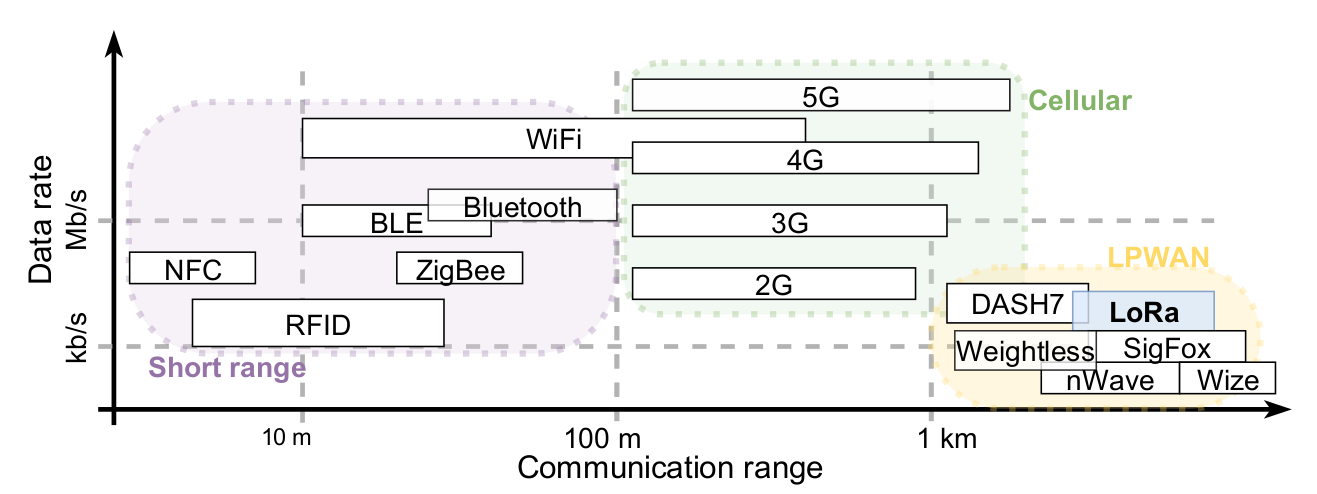
\includegraphics[height=4cm]{Figures/TechComparative.png}
        \caption[Comparision between communication technologies]{Comparison between different wireless communication technologies.}
        \cite{StarOfStars}
        \label{fig:TechComparative}
\end{figure}


LoRa, which stands for \textit{long range}, is a wireless communication technology owned by Semtech that operates in the sub-gigahertz range of the radio spectrum, specifically in the license-exempt Industrial, Scientific, Medical bands (ISM). It employs Chirp Spread Spectrum (CSS), a proprietary modulation technique resistant to multi-path fading and suitable for noisy environments, aiming to provide low throughput communication with links of more than 10 km –outdoors, in rural areas– while maintaining low power consumption.\cite{Augustin2016}

The amount of chirp that is used in the transmission is determined by the Spread Factor (SF) and this element is what makes LoRa interesting as by increasing this parameter the potential range increases at the expense of lower data throughput. 
LoRa also uses Forward Error Correction\footnote{\url{https://en.wikipedia.org/wiki/Error\_correction\_code\#Forward\_error\_correction}} (FEC) which helps with the robustness of the transmissions, specially in noisy environments.
As seen in \autoref{tab:ConfParamLoRa} LoRa is able to adapt to different scenarios by modifying its physical layer parameters: radio band and frequency, transmission power, bandwidth, FEC rate and SF although certain configurations may be against the radioelectric spectrum regulations in some jurisdictions.

\begin{table}[]
\centering
\begin{tabular}{|c|c|}
\hline
Configurable parameter & Values                    \\ \hline
Radio band             & 169, 433, 868, 915 MHz$^{a}$  \\ \hline
Bandwidth              & 62.5, 125, 250, 500 kHz$^{b}$ \\ \hline
Transmission power     & 14 dBm (EU), 27 dBm (USA) \\ \hline
Spreading Factor       & 6 to 12$^{c}$                 \\ \hline
FEC rate               & 4/5, 4/6, 4/7, 4/8        \\ \hline
\end{tabular}
\caption[Configurable parameters in LoRa transmissions]{Configurable parameters in LoRa transmissions \\
$^{a}$  Common frequency allocations for ISM in different regions worldwide; LoRa may also be used in licensed bands. \\
$^{b}$  Smaller bandwidths (7.8 to 41.7 kHz) are also supported, although rarely used. \\
$^{c}$  Certain bandwidth and SF combinations may result in too long transmissions for specific radio bands in which time-on-air limitations often apply.}
\label{tab:ConfParamLoRa}
\cite{StarOfStars}
\end{table}

Because LoRa is just a physical layer solution, LoRaWAN was invented to provide the MAC layer with a star topology, in which the regular nodes transmit their data in a single hop to the LoRaWAN gateway which in turn transmits it to the cloud through regular TCP/IP so the data can be later processed, be it for mathematical analysis or to distribute it to other nodes. This topology has several advantages, but also some inconvenients, as all the nodes that want to have connectivity need to be in physical range of a gateway, which will sometimes be technically or economically inviable.





%The reason that we chose LoRa for this subject is its low power consumption, its high range and the spread availability of LoRa integrated boards in the market, which, in turn, makes it affordable and easy to develop on as well as the proven reliability of the technology.
\subsubsection{Embedded devices: T-Beam}
In situations where LoRa is a suitable candidate for the communications of a solution, it is often common as well that small and a low power device is used. Thus we need to look for embedded systems that fulfill this requirements.

A common embedded board this days is the Raspberry Pi, which offers a high performance board for its size with the arm CPU architecture. It is also cheap –between 10 and 40\euro \ a piece, depending on the model– and it seems like an obvious choice to any project. However, there is some specific tasks in which a Raspberry does not perform good enough. Specifically when energy is a concern as it's estimated that it takes around 2 W\cite{PiConsumption} just to idle, and without a proper Power Management Unit (PMU) these boards also use 0.1 W when they are supposed to be shut down in addition to not support a proper sleep mode so they can we woken up later to perform periodic tasks\footnote{It is still possible to mount what's called a \textit{hat}, a physical add-on that could add the functionality of remote boot}. To put this energy measurements into perspective, a current smartphone battery would last a little bit more than half a day, thus requiring a solution to either replace the battery every one or two days –something rarely suitable– or extra hardware to provide constant energy, such as a solar cell, adding cost and complexity to the project.

Another common candidate for such tasks would be a single-board microcontroller, or what's commonly known as an \textit{Arduino}. These boards usually have lower processing power and resources but they tend to excel in the power management department which makes them great for IoT. In addition, finding one board with the exact features a project needs is relatively easy. This is the path we took. The board chosen is the TTGO T-Beam\footnote{\url{http://www.lilygo.cn/prod_view.aspx?TypeId=50033&Id=1163}}, a ESP32 SoC based board developed by LilyGo that provides us with a LoRa transceiver, WiFi+Bluetooth, a GPS as well as a hall sensor, highly programmable pins and the possibility to use a small display

\subsection{The problem}
% Aquests dos paràgrafs s'assemblen més a la "Justification" que no pas a "The problem" pero és que en certa manera tot està relacionat
During all of the history of humanity certain natural disasters have caused massive damage to properties, infrastructure, or even worse, the loss of lives; and even though predicting such events keeps being a challenging task this is not where the problems end. Rescue efforts, an extremely time critical task, and later on reconstruction work, usually rely on already existing infrastructure to assist them, but in such cases, infrastructures can not be relied upon as those probably have suffered the same fate. Thus, there is a need for a rapid deployment of critical infrastructure so relief efforts can act with the maximum efficiency without losing any second.\cite{LoRaMoto}

This is not the only use case of reliable distributed long range networks that exists. As mentioned in \cite{StarOfStars}, certain situations make it difficult to deploy a gateway close enough to a node or we would need as many gateways as nodes, which would make the use of LoRa completely pointless.


\begin{figure}[h]
        \centering
        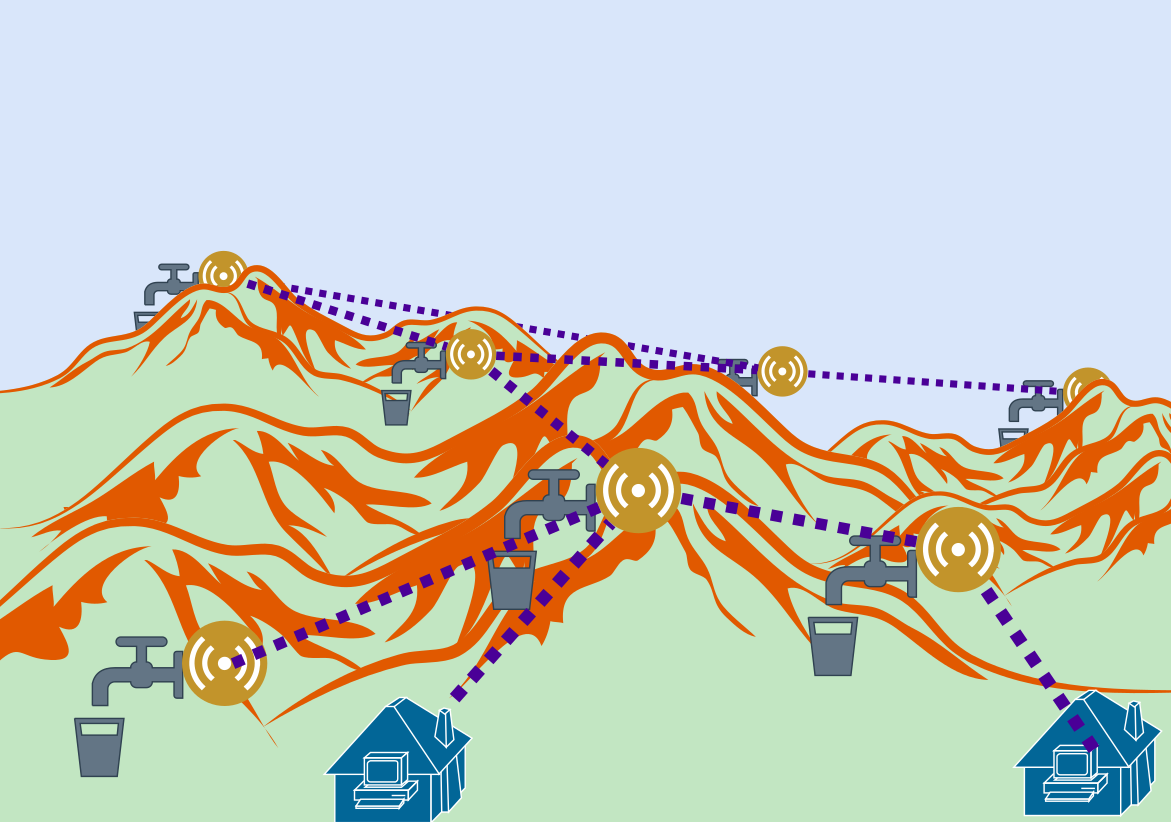
\includegraphics[height=5cm]{Figures/MountainMesh.png}
        \caption[Example of sparse network]{Example of sparse network. LoRaWAN gateways would need to be installed close to every node as one gateway wouldn't be able to have a data link to many nodes.}
        \cite{StarOfStars}
        \label{fig:MountainMesh}
\end{figure}


In this cases we need to  change the paradigm, stop using the star-shaped network and use a network that is able to use all the nodes it requires to transmit data in order to be reliable and cost effective, in other words, a \textit{mesh network}, where there is no central node governing all the others and it's all the nodes that work together by forming multi-hop paths so packets get to their final destination. This technology has been already developed and a clear and practical case is Meshtastic\footnote{\url{https://meshtastic.org}}, a communication tool that leverages mesh networking and GPS data to keep people in contact in rough environments.
However, in this case we will use a networking library developed by Roger Pueyo\footnote{\url{https://dsg.ac.upc.edu/user/149/biblio}}
The research will focus on evaluating and benchmarking his network routing protocol in different environments –urban/rural, noisy/quiet, dense/sparse– and different metrics such as the network throughput, RTT, or time to settle will be measured. In addition, to measure such metrics, we will have to develop appropriate tools that are able to carry the task and we will need to fit those tools into the microcontrollers.



\subsection{Stakeholders}
The actual uses of the research are multiple and we can classify the stakeholders of the project into four categories:
\begin{itemize}
\item \textbf{End users}: This group of individuals will be the one who probably benefits of the direct results of the research and sees it applied in the field with measurable improvements on performance and reliability. It's important to acknowledge that only those projects that need networks of sensors or actuators with a big dispersion between the nodes, without the need of lots of throughput and with no direct connection to the Internet will actually benefit from that. This group includes individual civilians as well as companies and public organizations.
\item \textbf{The university, UPC}: This entity has an academic interest in this project. UPC is interested to know if it can publish the research. In addition, UPC is in charge of overseeing the documentation of this project and provides a director to ensure quality and give prover guidance. 
\item \textbf{Distributed Systems Group (UPC)}\footnote{\url{https://dsg.ac.upc.edu}}: The research will be based on Roger's work for his ongoing PhD in the DSG about developing and studying mesh networks. It will provide them information on the performance and possible areas of optimization of the protocol he designed and implemented and it will also give insight on the reliability and ensure it can be used in real world scenarios. 
\end{itemize}

%Possibles entitats que desitgin desplegar un sistema distribuit de sensors i actuadors amb baixa densitat de nodes que no requereixi un throughput molt gran i que no tinguin conexio a internet
%Els usuaris que es beneficiaran de un potencial desplegament (mes enllà de la institució)
%La UPC, perque és la universitat que porta el projecte
%En Roger, perque l'ajuda a entendre millor el protocol

    \section{Justification}
    As mentioned before, there are some use cases where a long range low power mesh network is the most viable solution. However, even though this technology has been growing in the past years, there isn't a flexible implementation that is user friendly, moreso when it comes to a mesh protocol that doesn't rely on flooding the network with the message so the reciever gets the packet\cite{MeshtasticProto} rather than try to optimize the multi-hop protocol so the data only gets relied towards the direction of the final node. Thus, Roger's work will be one of the firsts to publicly design such protocol and with my help we will develop an implementation that satisfies such needs.


%In this cases we need to  change the paradigm and use a network that is able to use all the nodes it requires to transmit data in order to be reliable and cost effective, or what's called a \textit{mesh network}, where there is no central node governing all the other nodes, but it's every node that takes autonomous decisions to make sure it sends the data packets in the correct direction\footnote{Note that we are not talking about physical direction but more \textit{make good use of the resources available} direction}

    \section{Scope}
    We initially planned to do a performance analysis on the code that we had to develop on the first place but due to unforeseen circumstances the code is not to the final spec, which makes spending time doing a performance analysis a waste of resources as the code still needs some changes that will impact the functionality and the performance


\subsection{General objectives} \label{General objectives}
Because the focus of this research has been put into having a viable product rather than performing the analysis expected in the beginning, the final objectives have changed radically:
\subsubsection{Reliability}
Communications can range between two people sending pictures of cats to highly-critical and time sensitive information. It's important to accommodate all situations and make sure the messages get to the desired destinations.
\subsubsection{User friendliness and low profile}
The communications library should be easy to incorporate to any existing code without much refactoring and it should also be easy to create new programs that use the library without much trouble. In addition, the implementation needs to be easy on the few resources that the devices this code is going to run on have and shouldn't add too much processing overhead.
\subsubsection{Flexibility}
The library should be able to run in different architectures to provide wider compatibility across the ecosystem of IoT

%\subsection{Requirements}

% Functional and non functional requirements. Lo que sigui que aixo vol dir





%Desenvolupar eina de mesura
	% - Convertir el codi del Roger en una llibreria de veritat
	
%Planificar testbeds
%Executar proves
%Analitzar dades pertinents

%Mencionar que els riscs son basicament de temps i no de tecnologia i és que s'està fent analitzant una cosa que funciona
%Mencionar que has comprat una placa de debug (ESP-PROG) per a accelerar el development i que no hi hagi tantes incognites

%Posar les preguntes del Felix del document word
    \section{Methodology and rigor}
    Even thought the scope of the project has changed, the methodology and rigor stay mostly the same. The only changes are the deletion of the items related to the performance analysis. In addition, we will also be adding a logging functionality to ease the debugging.
    \section{Tasks}
    %Nivell de detall
%Estimacions en hores
%Ordre i dependències
%Recursos humans i materials
%Taula resum de les tasques
\label{sec:Tasks}
The research will happen between the months of February and June of 2021 and it's important to establish a reasonable time schedule to not lose track of progress and get stuck in secondary tasks that don't contribute significant results.

%Enumerar les tasques i subtasques i descriure-les
%Estimar les hores
%Anomenar les dependencies
%Fer una taula
All the work involved in the project will be mentioned here, as well as a simple explanation and the dependencies each task has on other tasks. Work not directly related on the project, such as familiarization with the tools used will also be mentioned here.

The schedule has been modified to accommodate the new objectives and the previous ones related to the analysis have been removed


\subsection{Researching and Learning phase}
% Buscar quines plataformes fer servir
	% Instalar VSCOD
	% Instalar PlatformIO
	% Instalar
% Familiartizar-se amb les tecnologies
% Fer PoC per demostrar la viablitiat

Prior to starting the research some work on familiarizing with the technologies will be done. This is an important step to ensure good results and to find problems early on that could impact the project viability later on. \autoref{tab:InitialTasks} shows the tasks related as well as its dependencies and resources associated with them:

\begin{table}[ht]
\centering
\resizebox{\textwidth}{!}{%
\begin{tabular}{|c|l|c|c|c|}
\hline
\rowcolor[HTML]{9B9B9B} 
\multicolumn{1}{|c|}{\cellcolor[HTML]{9B9B9B}\textbf{ID}} &
  \multicolumn{1}{c|}{\cellcolor[HTML]{9B9B9B}\textbf{Description}} &
  \multicolumn{1}{c|}{\cellcolor[HTML]{9B9B9B}\textbf{\begin{tabular}[c]{@{}c@{}}Work\\ Hours\end{tabular}}} &
  \multicolumn{1}{c|}{\cellcolor[HTML]{9B9B9B}\textbf{Resources}} &
  \multicolumn{1}{c|}{\cellcolor[HTML]{9B9B9B}\textbf{Deps.}} \\ \hline
  \rowcolor[HTML]{C0C0C0}
T1 &
  \begin{tabular}[c]{@{}l@{}}\textbf{Software Installation}\\ Install all the necessary tools to perform the research activities\end{tabular} &
   6&
   
\includegraphics[height=4mm]{Figures/laptop_emoji.png}&
   \\ \hline
T1.1 &
  \begin{tabular}[c]{@{}l@{}}\textbf{Install VSCode}\\ Install the IDE we are going to use to develop the code\end{tabular} &
   4&
   
\includegraphics[height=4mm]{Figures/laptop_emoji.png}&
   \\ \hline
T1.2 &
  \begin{tabular}[c]{@{}l@{}}\textbf{Install PlatformIO}\\ Install the add-on we are going to use to interface with the board\end{tabular} &
   2&
   
\includegraphics[height=4mm]{Figures/laptop_emoji.png}&
  T1.1 \\ \hline
  \rowcolor[HTML]{C0C0C0}
T2 &
  \begin{tabular}[c]{@{}l@{}}\textbf{Familiarizing with PlatformIO and the TTGO Board}\\ Make sure I'm able to confidently develop and debug software on the\\current setup\end{tabular} &
   35&
   
\includegraphics[height=4mm]{Figures/laptop_emoji.png}
   
\includegraphics[height=4mm]{Figures/microcontroller_emoji.png}&
  T1 \\ \hline
T2.1 &
  \begin{tabular}[c]{@{}l@{}}\textbf{Reading documentation on the ESP32 collection of libraries}\\ ESP32 has a large amount of features divided between different libraries. \\ Understanding the basic functionalities of the board is essential to \\use all the features in a smart way\end{tabular} &
   10&
   &
   \\ \hline
T2.2 &
  \begin{tabular}[c]{@{}l@{}}\textbf{Reading documentation on TTGO Board}\\ Understand what features the board has and how to use them\end{tabular} &
   5&
   &
   \\ \hline
T2.3 &
  \begin{tabular}[c]{@{}l@{}}\textbf{Reading documentation on PlatformIO}\\ Make sure I follow the most efficient procedures the add-on offers\end{tabular} &
   10&
   &
   \\ \hline
T2.4 &
  \begin{tabular}[c]{@{}l@{}}\textbf{Testing the knowledge aquired}\\ Develop small programs to test all the features that could be useful for the\\research\end{tabular} 	   &
   10&
   
\includegraphics[height=4mm]{Figures/laptop_emoji.png}
   
\includegraphics[height=4mm]{Figures/microcontroller_emoji.png}&
  \begin{tabular}[c]{@{}l@{}}T2.1\\ T2.2\\ T2.3\end{tabular} \\ \hline
  \rowcolor[HTML]{C0C0C0}
T3 &
  \textbf{Develop feature rich PoC to make sure I'm ready to start developing} &
   30 &
   
\includegraphics[height=4mm]{Figures/laptop_emoji.png}
   
\includegraphics[height=4mm]{Figures/microcontroller_emoji.png}&
  T2 \\ \hline
\end{tabular}%
}
\caption{List of tasks for the Researching and Learning phase}
\label{tab:InitialTasks}
\end{table}


\subsection{Conception and Initiation phase}
% Documentacio preliminar
% Traçar un full de ruta
% Preveure obstacles
% En general copiar lo de l'Aaron
Defining a roadmap is essential to have a well defined project that is easy to manage and complete. This section explains the tasks related to the management and planning of the project in its first stages.\autoref{tab:DocumentationTasks} shows the tasks related as well as its dependencies and resources associated with them: 

\begin{table}[ht]
\centering
\resizebox{\textwidth}{!}{%
\begin{tabular}{|c|l|c|c|c|}
\hline
\rowcolor[HTML]{9B9B9B} 
\textbf{ID} &
  \multicolumn{1}{c|}{\cellcolor[HTML]{9B9B9B}\textbf{Description}} &
  \textbf{\begin{tabular}[c]{@{}c@{}}Work\\ Hours\end{tabular}} &
  \textbf{Resources} &
  \textbf{Deps.} \\ \hline
\rowcolor[HTML]{C0C0C0} 
T4 &
  \begin{tabular}[c]{@{}l@{}}\textbf{Inititial scope}\\ Study the basics of the project and have a good understanding of\\ what sorounds it\end{tabular} &
   26&
   &
  T2 \\ \hline
T4.1   & \begin{tabular}[c]{@{}l@{}}\textbf{Project Context}\\ Define the different topics the project will interact with\end{tabular}                   & 14 &  &    \\ \hline
T4.1.1 & \begin{tabular}[c]{@{}l@{}}\textbf{Academic Context}\\ Define how the research fits into the current academic setting\end{tabular}              & 4 &  &    \\ \hline
T4.1.2 & \begin{tabular}[c]{@{}l@{}}\textbf{Terms and concepts}\\ Define the technologies and resources used in the research\end{tabular}                & 4 &  &    \\ \hline
T4.1.3 & \begin{tabular}[c]{@{}l@{}}\textbf{The problem}\\ Define the problem that wants to be solved by the research\end{tabular}                       & 4 &  &    \\ \hline
T4.1.4 & \begin{tabular}[c]{@{}l@{}}\textbf{Stakeholders}\\ Investigate the actors interested in the research\end{tabular}                               & 2 &  &    \\ \hline
T4.2 &
  \begin{tabular}[c]{@{}l@{}}\textbf{Project Justification}\\ Justify why the research is needed and how it differs from previous ones\end{tabular} &
   2&
   &
  T4.1.3 \\ \hline
T4.3   & \begin{tabular}[c]{@{}l@{}}\textbf{Project Scope}\\ Define what the project is and is not\end{tabular}                                          & 6 &  &    \\ \hline
T4.3.1 & \begin{tabular}[c]{@{}l@{}}\textbf{General Objectives}\\ Define the goals of the research\end{tabular}                                          & 4 &  &    \\ \hline
T4.3.2 & \begin{tabular}[c]{@{}l@{}}\textbf{Risk Assessment}\\ Investigate possible issues that may arise during the course of the research\end{tabular} & 2 &  &    \\ \hline
T4.4   & \begin{tabular}[c]{@{}l@{}}\textbf{Methodology and Rigor}\\ Define methodologies and tools that will help obtain reliable results\end{tabular}  & 4 &  & T2 \\ \hline
T4.4.1 & \begin{tabular}[c]{@{}l@{}}\textbf{Programming workflow}\\ Define the set of procedures that will ensure a bug-free code\end{tabular}             & 2 &  &    \\ \hline
\rowcolor[HTML]{C0C0C0} 
T5 &
  \begin{tabular}[c]{@{}l@{}}\textbf{Review the documentation}\\ Make sure all sections make sense between each other and comment the\\text with the directors\end{tabular} &
   8&
   
\includegraphics[height=4mm]{Figures/teacher_emoji.png}&
  T4 \\ \hline
  \rowcolor[HTML]{C0C0C0} 
T6 &
  \begin{tabular}[c]{@{}l@{}}\textbf{Task analysis}\\ Identify and organize the tasks and subtasks that are going to be part\\of this project\end{tabular} &
   4&
   &
  T5 \\ \hline
  \rowcolor[HTML]{C0C0C0} 
T7 &
  \begin{tabular}[c]{@{}l@{}}\textbf{Project Planning}\\ Estimate the time needed for each task and its dependencies\end{tabular} &
   4&
   &
  T6 \\ \hline
  \rowcolor[HTML]{C0C0C0} 
T8 &
  \begin{tabular}[c]{@{}l@{}}\textbf{Sustainability analysis}\\ Estimate the impact of the project to the environment and society\end{tabular} &
   6&
   &
  T5 \\ \hline
\end{tabular}%
}
\caption{List of tasks for the Conception and Initiation phase}
\label{tab:DocumentationTasks}
\end{table}

\subsection{Design and Implementation phase}
% Convertir el codi a llibreria
% Adaptar la llibreria per tenir acces de lectura a les estructures internes
% Dissenyar estructura del programa
% Implementar mecanisme de sincronitzacio entre nodes
% Implementar la recoleccio de dades
	% Local
	% Internet
% Dissenyar tipus de tests
% Implementar la generacio de tests (Possiblement de forma dinamica)

The first step once there is a clear roadmap is to start preparing the right environment for the experiments, designing and implementing the tools needed. \autoref{tab:ProgramingTasks} shows the tasks related as well as its dependencies and resources associated with them:

The next step after we have a clear roadmap is to set up a good developing environment to speed up code development. In this section we will find some unforeseen circumstances that will delay the implementation.

\begin{table}[ht]
\centering
\resizebox{\textwidth}{!}{%
\begin{tabular}{|c|l|c|c|c|}
\hline
\rowcolor[HTML]{9B9B9B} 
\textbf{ID} &
  \multicolumn{1}{c|}{\cellcolor[HTML]{9B9B9B}\textbf{Description}} &
  \textbf{\begin{tabular}[c]{@{}c@{}}Work\\ Hours\end{tabular}} &
  \textbf{Resources} &
  \textbf{Deps.} \\ \hline
\rowcolor[HTML]{C0C0C0} 
T9 &
  \begin{tabular}[c]{@{}l@{}}\textbf{Make ESP-Prog work on the T-Beam}\\ The documentation was incorrect and the ESP-Prog  needs some additional \\ work to be useful\end{tabular} &
   40&
   	
\includegraphics[height=4mm]{Figures/laptop_emoji.png}
	
\includegraphics[height=4mm]{Figures/microcontroller_emoji.png}
	
\includegraphics[height=4mm]{Figures/screwdriver_emoji.png}&
  T5 \\ \hline
\rowcolor[HTML]{C0C0C0} 
T10 &
  \begin{tabular}[c]{@{}l@{}}\textbf{Decide which parts of the code are relevant}\\ The PoC is operational but there's bloat that needs to be removed. \end{tabular} &
   20&
   	
\includegraphics[height=4mm]{Figures/laptop_emoji.png}
	
\includegraphics[height=4mm]{Figures/teacher_emoji.png}&
   \\ \hline
\rowcolor[HTML]{C0C0C0} 
T11 &
  \begin{tabular}[c]{@{}l@{}}\textbf{Design library architecture}\\ Research and design a architecture for the library and how its different\\pieces will interact with each other\end{tabular} &
   20&
      
\includegraphics[height=4mm]{Figures/laptop_emoji.png}
&
   T10 \\ \hline
   \rowcolor[HTML]{C0C0C0} 
T12 &
  \begin{tabular}[c]{@{}l@{}}\textbf{Implement library}\\ Implement the library in C++ and make use of OOP\end{tabular} &
   140&
   
\includegraphics[height=4mm]{Figures/laptop_emoji.png}
	
\includegraphics[height=4mm]{Figures/microcontroller_emoji.png}
	
\includegraphics[height=4mm]{Figures/screwdriver_emoji.png}&
   T11\\ \hline
T12.1 &
  \begin{tabular}[c]{@{}l@{}}\textbf{Solve hardware architecture problems}\\ The hardware architecture is more complex than initially thought\end{tabular} &
   40&
   
\includegraphics[height=4mm]{Figures/laptop_emoji.png}
	
\includegraphics[height=4mm]{Figures/microcontroller_emoji.png}
	
\includegraphics[height=4mm]{Figures/screwdriver_emoji.png}&
   \\ \hline
T12.2 &
  \begin{tabular}[c]{@{}l@{}}\textbf{Solve software issues}\\ FreeRTOS and Radiolib are two complex libraries that require special care\end{tabular} &
   60&
   
\includegraphics[height=4mm]{Figures/laptop_emoji.png}
	
\includegraphics[height=4mm]{Figures/microcontroller_emoji.png}
	
\includegraphics[height=4mm]{Figures/screwdriver_emoji.png}&
   \\ \hline
\rowcolor[HTML]{C0C0C0} 
T13 &
  \begin{tabular}[c]{@{}l@{}}\textbf{Testing}\\ Testing will be conducted through the whole coding process\end{tabular} &
   80&
   	
\includegraphics[height=4mm]{Figures/laptop_emoji.png}
	
\includegraphics[height=4mm]{Figures/microcontroller_emoji.png}
	
\includegraphics[height=4mm]{Figures/screwdriver_emoji.png}&
  T11 \\ \hline
\end{tabular}%
}
\caption{List of tasks for the Design and Implementation phase}
\label{tab:ProgramingTasks}
\end{table}

% Fer que el ESP-Prog funcioni
% Analitzar llibreria i veure què es queda i què s'enva
% Pensar en la arquitectura de la llibreria
% Passar el codi a C++ i OOP
%% Solucionar problemes amb l'arquitectura (lo de les funcions en instancies)
%% Solucionar problemes de FreeRTOS i RadioLib
% Testing (dir que s'incorpora en les tasques anteriors)






\subsection{Closing phase}
% Documentation wrap up
% Presentation

\autoref{tab:WrapupTasks} shows the tasks related the final stages of the research as well as its dependencies and resources associated with them:

\begin{table}[]
\centering
\resizebox{\textwidth}{!}{%
\begin{tabular}{|c|l|c|c|c|}
\hline
\rowcolor[HTML]{9B9B9B} 
\textbf{ID} &
  \multicolumn{1}{c|}{\cellcolor[HTML]{9B9B9B}\textbf{Description}} &
  \textbf{\begin{tabular}[c]{@{}c@{}}Work\\ Hours\end{tabular}} &
  \textbf{Resources} &
  \textbf{Deps.} \\ \hline
\rowcolor[HTML]{C0C0C0} 
T14 &
  \begin{tabular}[c]{@{}l@{}}\textbf{Documentation wrap up}\\ Make sure the final document is understandable and every \\important topic has been explained in detail. In addition,\\properly format the document and create visual assets\end{tabular} &
   60 &
   
\includegraphics[height=4mm]{Figures/laptop_emoji.png}
   
\includegraphics[height=4mm]{Figures/teacher_emoji.png}&
  T13 \\ \hline
\rowcolor[HTML]{C0C0C0} 
T15 &
  \begin{tabular}[c]{@{}l@{}}\textbf{Presentation}\\ Prepare a visual presentation to show the research to the comitee\end{tabular} &
   40 &
   
\includegraphics[height=4mm]{Figures/laptop_emoji.png}
   
\includegraphics[height=4mm]{Figures/teacher_emoji.png}&
  T14 \\ \hline
\end{tabular}%
}
\caption{List of tasks for the Closing phase}
\label{tab:WrapupTasks}
\end{table}


% Please add the following required packages to your document preamble:
% \usepackage{graphicx}
% \usepackage[table,xcdraw]{xcolor}
% If you use beamer only pass "xcolor=table" option, i.e. \documentclass[xcolor=table]{beamer}
\begin{table}[]
\centering
\resizebox{\textwidth}{!}{%
\begin{tabular}{|c|l|}
\hline
\rowcolor[HTML]{C0C0C0} 
\multicolumn{1}{|l|}{\cellcolor[HTML]{C0C0C0}ID} & Description                                                                 \\ \hline

\includegraphics[height=4mm]{Figures/laptop_emoji.png} & Fully working workstation                                                   \\ \hline

\includegraphics[height=4mm]{Figures/microcontroller_emoji.png}  & TTGO T-Beam board. The amount of boards needed will vary during development \\ \hline

\includegraphics[height=4mm]{Figures/teacher_emoji.png} & The directors of the project. They offer great advice                       \\ \hline

\includegraphics[height=4mm]{Figures/screwdriver_emoji.png} & ESP-Prog. The debugging board. We will only need one                        \\ \hline
\end{tabular}%
}
\caption{Legend of Resources}
\label{tab:Resources}
\end{table}

\subsection{Modifications implications}
Overall, the modifications in the tasks add 18h more of work as the development of the library took way more time than initially planned. The time increase, however, does not make the project impossible to perform in the expected schedule.
%%En total son 461h+18h o 25h/ECTS






    %\section{Gantt}
    %The following is a representation of the tasks with Gantt graphs, its expected that the work is done on weekdays at 8 h of work a day. The figures don't account for possible holidays for software limitations. In addition the project is expected to be finished before schedule. This is to accommodate probable delays in software development or the experiments. Figures \ref{fig:GanttRLCI}, \ref{fig:GanttSIP} and \ref{fig:GanttTAC} show the schedule defines according to Section \ref{sec:Tasks}

\begin{figure}[h]
        \centering
        \centerline{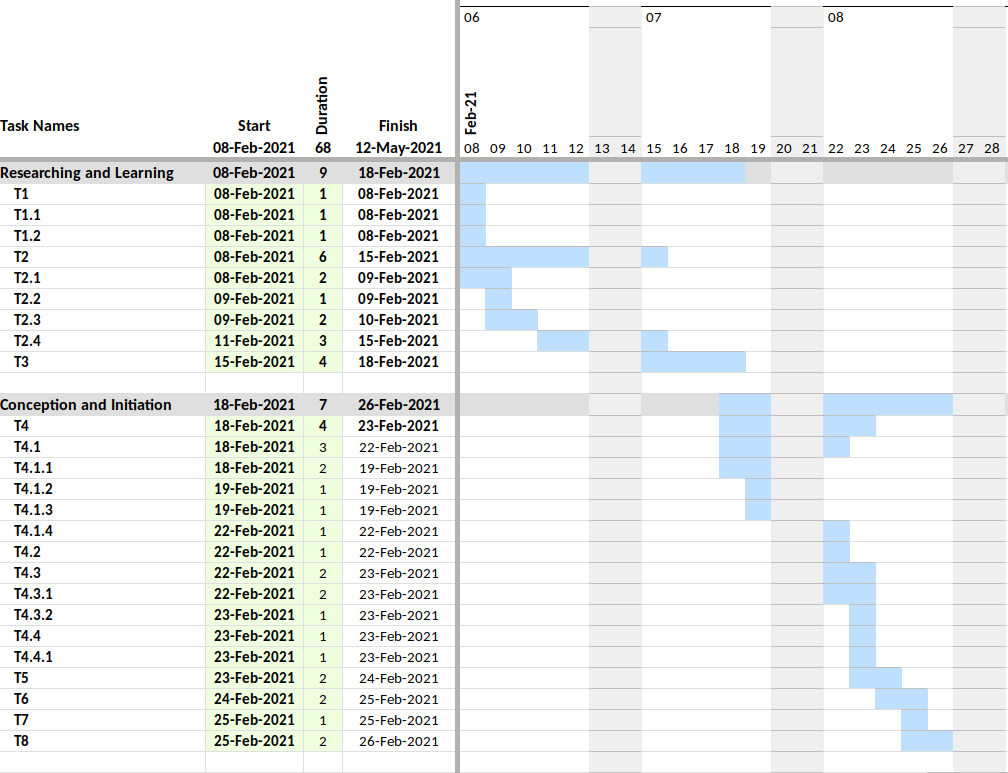
\includegraphics[scale=0.45]{Figures/Gantt_RL_and_CI.png}}
        \caption{Gantt of the first two sections: \textit{Research and Learning} and \textit{Conception and Initiation}}
        \label{fig:GanttRLCI}
\end{figure}

\begin{landscape}

\begin{figure}[ht]
        \centering
        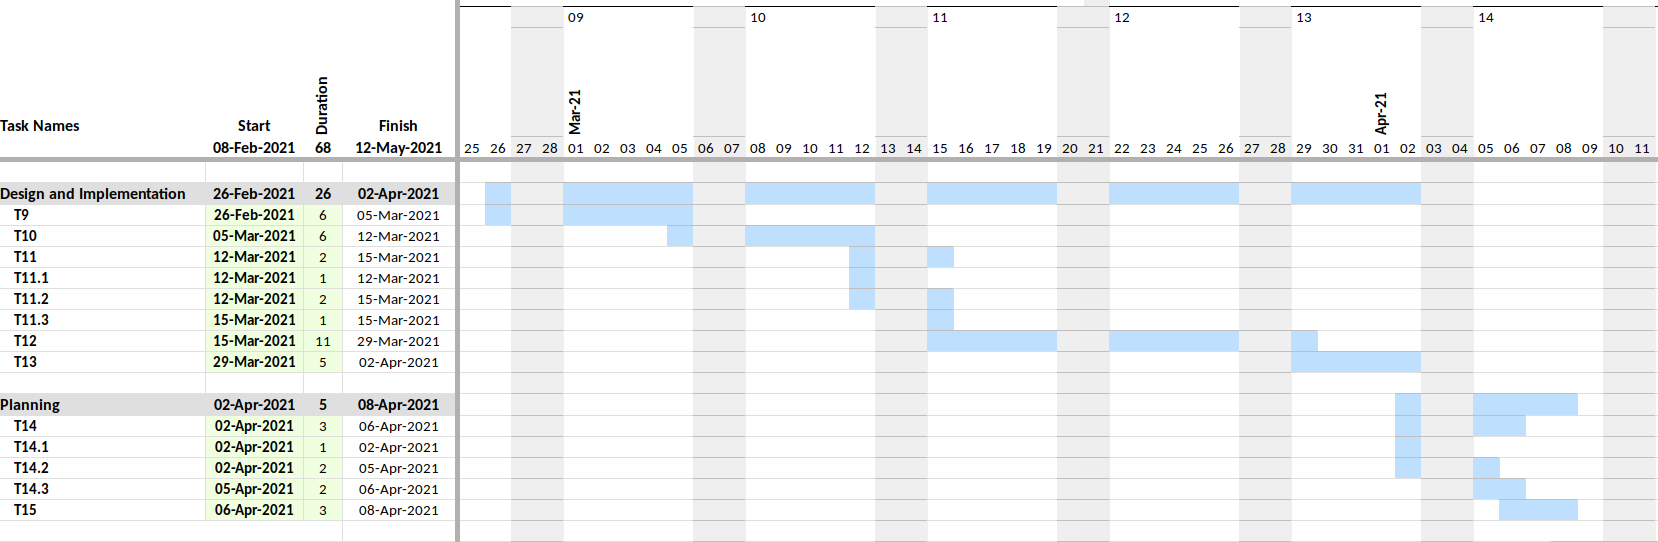
\includegraphics[scale=0.27]{Figures/Gantt_SI_and_P.png}
        \caption{Gantt of the middle two sections: \textit{Design and Implementation} and \textit{Planning}}
        \label{fig:GanttSIP}
\end{figure}

\begin{figure}[ht]
        \centering
        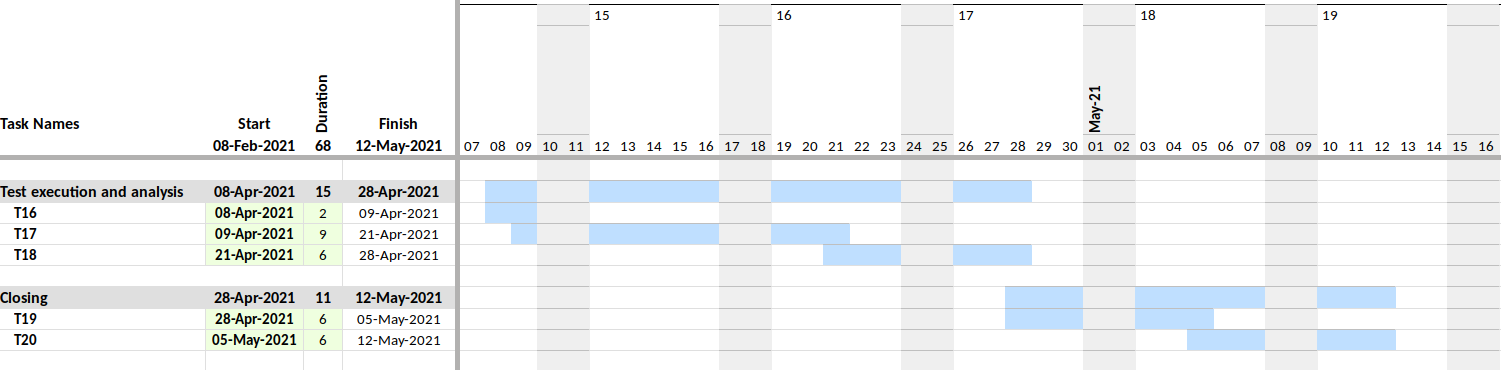
\includegraphics[scale=0.29]{Figures/Gantt_TA_and_C.png}
        \caption{Gantt of the middle two sections: \textit{Test execution and analysis} and \textit{Closing}}
        \label{fig:GanttTAC}
\end{figure}

\end{landscape}
    \section{Risk management}
    Every project has expected and unexpected issues and it's important to plan ahead to make sure certain circumstances affect the least amount to the correct development of the research, thus we need to foresee those circumstances and take the necessary measures for them to not happen or to be able to continue without a big delay. The following is a non-exhaustive list of the problems that may arise:
\subsection{Time predictions and objective overshooting}
Having too complex objectives may delay the end date of the project, not reaching the proposed deadline. Thus, it's important to have flexible and modular objectives that can be added or removed without great impact to the quality of the research but that at the same time allow the deadline to be reached. In this case we ended up aiming for a project that was too complex and we had to reconsider the objectives.

\subsection{Unexpected implementation delays}
Software development is known for taking longer than originally planned. It's paramount to have good coding practices, such as unit testing, using version control tools how they are supposed to be used and having good code quality overall trying to avoid code smells. In addition, the board ESP-Prog will allow to debug the code in the microcontroller as if it was running on our workstation, something that will speed up debugging time significantly. However, as it turned out trying to set up this up contributed to the delay of the project.

    \section{Sustainability}
    \textit{Infinite growth in a finite world is impossible}. We all heard this sentence once in our lifetimes and it is important to remind us of it from time to time when we try to use the resources available to us. When we design a project like this it is not only important to estimate the direct benefits it will have but also what are the implications in the long term or on remote places.
IT is known for its many technological resources and potential impact on the life of everyone but the concept of \textit{social justice} must not be forgotten and it needs to be taken into account during the design and implementation phase of any project to not create more inequality or borrow resources that will never get put back in place, further expanding the breach between poor and rich areas or creating division within communities.

As engineers we have the responsibility of creating systems that relieve people from tasks and improve their lives and try to minimize the negative effects or even reconsider the whole project if those outweigh the benefits.

\subsection{Environmental Sustainability}
The proposed implementation of the project uses relatively few resources. Apart from a workstation --something that most projects nowadays require-- a few small boards are needed. However, it's worth noting that this tools have a significant impact due to the ores needed to manufacture silicon and the ways of extraction as well as the transportation of the devices across the world for assembly and distribution --for example, the ESP-Prog board was shipped from China in 10 days--. On the other hand, because I use my own computer I get to decide where to source it from and in this case it's second hand, but this is not applicable in a business setting where buying equipment second hand is rarely done.

The project strives to make telecommunication more efficient which should, in turn reduce the resources needed to provide connectivity to remote nodes that currently use more resources, be it for energy consumption or infrastructure that could be superseded by the knowledge of the research. However, we need to acknowledge the Jevons' paradox\cite{Alcott2005} which states that improvements in efficiency do not imply a reduced use of the resource but totally the opposite.

\subsection{Economical Sustainability}
The estimated cost of the complete process of the project is estimated to be 16644\euro\ as it will be seen in \autoref{sec:Total}.

Currently the field of LoRa Mesh is in its infancy and with great potential for development and optimization which makes this project an interesting topic with great opportunity for a return of investment as current implementations either use some technology like GSM, which is expensive and power requiring or, in case they use LoRaWan, the costs of setting up and maintaining the gateways significantly increases the costs of the installations. This research will try to put some light into mesh networking, specially for LoRa devices and make it open to the public so anyone can benefit from it or research on top of it.

\subsection{Social Sustainability}
I think this project is a great opportunity to get introduced to the research world at the same time I work with something that I have interest in. Because I have a great amount of flexibility, I expect this to give me the expertise in project management and problem-solving skills when facing issues during the project as well as a good insight in LoRa and mesh networking.

The project will have real implications in the field of telecommunications in remote areas where infrastructure is expensive to set up and maintain, thus allowing entities to save on costs, either economical or human, by automating some or all the tasks of certain processes, as presented in \cite{LoRaMoto}. Hopefully this research will help to save millions of euros in infrastructure and thousands of man-hours by providing --albeit small-- connectivity to remote or challenging places.
    \section{Budged and costs}
    Budgeting and properly managing the costs later in the project are important steps to take in order to stop possible mistakes in time and guarantee the success of the project. In the following sections we will explain the costs associated with the research and how they are distributed.
\subsection{Direct costs}
Direct costs are those consisting in human costs plus the amortization of all the hardware we will need. In order to have a good estimation of what would be the costs in an ordinary work environment we will pretend that the tasks will be done by different people with different roles within the organization, with a salary similar to what would be standard in Spain. Tables \ref{tab:Roles} and \ref{tab:Costs} show those costs.

To compute amortizations we will take into account the prices of the hardware devices we already had and compute the amortization costs during the research. We will estimate that all the electronic devices have a 5 year lifespan and apply the following formula to compute the amortization costs: $$ Cost = \dfrac{Retail Price}{\frac{Useful Life}{Time Used}} $$
\autoref{tab:AmortizationCosts} shows the amortization costs associated with the project. The total costs of this section amount to 10340\euro\ + 134\euro\ = 10474\euro, or 2330\euro cheaper than initially planned.

\begin{table}[ht]
\centering
\begin{tabular}{|c|l|c|c|c|}
\hline
\rowcolor[HTML]{9B9B9B} 
\textbf{Abbr.} &
  \multicolumn{1}{c|}{\cellcolor[HTML]{9B9B9B}\textbf{Role Name}} &
  \textbf{Hours} &
  \textbf{\begin{tabular}[c]{@{}c@{}}Salary\\ \euro/h\end{tabular}} &
  \textbf{Cost} \\ \hline
PA & Project Administrator & 148 & 30 & 4440  \\ \hline
SA & Software architect    & 40 & 24 & 960 \\ \hline
P  & Programmer            & 291 & 20 & 3980 \\ \hline
EE & Electrical Engineer   & 40 & 24 & 960 \\ \hline
\end{tabular}%
\caption{Costs associated with every role in the project.}
\label{tab:Roles}
\end{table}


% Please add the following required packages to your document preamble:
% \usepackage{graphicx}
% \usepackage[table,xcdraw]{xcolor}
% If you use beamer only pass "xcolor=table" option, i.e. \documentclass[xcolor=table]{beamer}
\begin{table}[ht]
\centering
\begin{tabular}{|c|c|c|c|c|c|c|c|c|c|c|}
\cline{1-5} \cline{7-11}
\cellcolor[HTML]{9B9B9B}\textbf{ID} &
  \cellcolor[HTML]{9B9B9B}\textbf{Role} &
  \cellcolor[HTML]{9B9B9B}\textbf{Hours} &
  \cellcolor[HTML]{9B9B9B}\textbf{\begin{tabular}[c]{@{}c@{}}Salary\\ \euro/h\end{tabular}} &
  \cellcolor[HTML]{9B9B9B}\textbf{Cost} &
  \textbf{} &
  \cellcolor[HTML]{9B9B9B}\textbf{ID} &
  \cellcolor[HTML]{9B9B9B}\textbf{Role} &
  \cellcolor[HTML]{9B9B9B}\textbf{Hours} &
  \cellcolor[HTML]{9B9B9B}\textbf{\begin{tabular}[c]{@{}c@{}}Salary\\ \euro/h\end{tabular}} &
  \cellcolor[HTML]{9B9B9B}\textbf{Cost} \\ \cline{1-5} \cline{7-11} 
T1  & P  & 6  & 20 & 120 & \textbf{} & T11 & SA & 20  & 24 & 480  \\ \cline{1-5} \cline{7-11} 
T2  & P  & 35 & 20 & 700 & \textbf{} & T12 & P  & 140 & 20 & 2800  \\ \cline{1-5} \cline{7-11} 
T3  & P  & 30 & 20 & 600 & \textbf{} & T13 & P & 80 & 20 & 1600  \\ \cline{1-5} \cline{7-11} 
T4  & PA & 26 & 30 & 780 & \textbf{} & T14 & PA & 60 & 30 & 180  \\ \cline{1-5} \cline{7-11} 
T5  & PA & 8  & 30 & 240 & \textbf{} & T15 & PA & 40 & 30 & 1200  \\ \cline{1-5} \cline{7-11} 
T6  & PA & 4  & 30 & 120 & \textbf{} &  &  &  &  &  \\ \cline{1-5} \cline{7-11} 
T7  & PA & 4  & 30 & 120 & \textbf{} &  &  &  &  &  \\ \cline{1-5} \cline{7-11} 
T8  & PA & 6  & 30 & 180 & \textbf{} &  &  &  &  &  \\ \cline{1-5} \cline{7-11} 
T9  & EE  & 40 & 24 & 960 & \textbf{} &  &  &  &  &  \\ \cline{1-5} \cline{7-11} 
T10 & SA  & 20 & 24 & 480 & \textbf{} &  &  &  &  &  \\ \cline{1-5} \cline{7-11} 
 &   &  &  &  &  \textbf{} & Total &  &  &  &  10340\\ \cline{1-5} \cline{7-11}
\end{tabular}%

\caption{Costs associated with every task. Taxes included}
\label{tab:Costs}
\end{table}


\begin{table}[ht]
\centering
\begin{tabular}{|c|c|c|c|c|}
\hline
\rowcolor[HTML]{9B9B9B} 
\textbf{Item} &
  \textbf{\begin{tabular}[c]{@{}c@{}}Unit\\ Cost \euro\end{tabular}} &
  \textbf{Units} &
  \textbf{\begin{tabular}[c]{@{}c@{}}Use\\ (mo)\end{tabular}} &
  \textbf{\begin{tabular}[c]{@{}c@{}}Cost\\ \euro\end{tabular}} \\ \hline
Workstation & 1700 & 1  & 4 & 113 \\ \hline
T-Beam      & 30   & 10 & 4 & 20 \\ \hline
ESP-Prog    & 15   & 1  & 4 & 1 \\ \hline
\end{tabular}%

\caption{Amortization costs}
\label{tab:AmortizationCosts}
\end{table}


\subsection{Indirect costs}
Indirect costs refer to the costs of a project, regardless of specifics. We identify electricity, Internet access and rent as such. In order to have a good approximation, we'll use a typical co-working space which averages\footnote{Used to, the pandemic changed the prices significantly} 300\euro\ in the city of Barcelona. Which for the whole duration of the project, four months, adds up to 1200\euro.

\subsection{Contingencies}
Contingency costs is the budged reserved to cover delays in development and an overall extensions of the project. We will allocate an extra 20\% for possible delays. This amounts to $(1200$\euro $+ 12670$\euro$) \times 0.2 = 2774$\euro  

\subsection{Incidentals}
Incidental costs are related to the occurrence of possible risks that usually do not depend on the people in charge of the project. In this case, disregarding the bus factor\footnote{\url{https://en.wikipedia.org/wiki/Bus\_factor}} little amount of incidents can occur that lead to more spending. There is no licensing whatsoever and the experiment schedules should be planned in a flexible way so restrictions don't affect the data gathering in a severe way

\subsection{Total}
\label{sec:Total}
If we add up the Direct costs, Indirect costs and Contingencies we obtain, as shown in \autoref{tab:TotalCosts} that the total budged for the project is 14314\euro\ or 2300\euro\ less than before

% Please add the following required packages to your document preamble:
% \usepackage{graphicx}
% \usepackage[table,xcdraw]{xcolor}
% If you use beamer only pass "xcolor=table" option, i.e. \documentclass[xcolor=table]{beamer}
\begin{table}[ht]
\centering
\begin{tabular}{|c|c|}
\hline
\rowcolor[HTML]{9B9B9B} 
\textbf{Type} & \textbf{\begin{tabular}[c]{@{}c@{}}Cost\\ \euro\end{tabular}} \\ \hline
Direct        & 10474                                                      \\ \hline
Indirect      & 1200                                                       \\ \hline
Contingencies & 2774                                                       \\ \hline
\rowcolor[HTML]{C0C0C0} 
Total         & 14314                                                      \\ \hline
\end{tabular}%

\caption{Project costs by category}
\label{tab:TotalCosts}
\end{table}

\subsection{Management Procedures}
In order to make sure the project does not go off the rails with uncountable delays it's important to detect them early on to apply the proper solutions. In order to keep track of a natural development of the project we will pay close attention to the Direct costs because it's where the greatest variance between the expected and the actual ---worked hours--- will be potentially greatest. We will use the following formula to know the cost deviation: $$ Cost Deviation = (Expected hours - Real Hours) \times Hour Rate $$
We can use this formula to know the overall Cost deviation but also apply the same formula to individual tasks to have a fine grained control of the situation.
    \section{•}
    % Parlar sobre les modificacions a la placa per adaptar el debugger
    % Parlar sobre passar instancies de una classe a la ISR (aprofitar per explicar què és una ISR)
    % Parlar sobre FreeRTOS
    % Parlar sobre problemes misteriosos
    	% Parlar sobre rebre paquets fantasma quan es transmet un paquet
    	% Parlar sobre diversos crashes en el sistema per culpa de les prioritats i rutines blocants (wdt)
    \section{Legal considerations}
    The scope of this project overlaps with several laws in the European Union regarding telecommunications and the use of the electromagnetic spectrum. It is important to have the appropriate considerations when dealing with laws and take the necessary measures to stay inside of the constraints these state. According to ETSI, an European standards organization, it is mandatory that no more than 1\% of the time averaging in 1h\cite{DutyCicle} is occupied transmitting and using the electromagnetic space for devices such as the ones we will be using and are in scope of the project.

Even though providing the proper code to make sure this is taken care of would be ideal, doing so while not compromising the objectives of having a user friendly library is more difficult as the only good implementation is one that is completely transparent to the end user, who may be unaware of the regulation or even that this kind of regulation exists. This feature is inside of the list of things to do in the future but currently the library needs the user to take care of this issue. In addition, \cite{DutyCicle} also states allowed transmitting powers and frequencies, however, this is mostly responsibility of the hardware or the end user, as they change slightly depending on the country but the hardware itself is compliant with CE\footnote{\url{https://en.wikipedia.org/wiki/CE_marking}} so it should never be allowed to operate in disallowed bands or powers.
    
	\newpage
    \bibliography{bibliography}
	\bibliographystyle{plain}
    
    
\end{document}
